
%(BEGIN_QUESTION)
% Copyright 2007, Tony R. Kuphaldt, released under the Creative Commons Attribution License (v 1.0)
% This means you may do almost anything with this work of mine, so long as you give me proper credit

Suppose we were to test the voltage at the source end of a long cable, driven by a 24 volt power supply and a fast-switching MOSFET transistor:

$$\includegraphics[width=15.5cm]{i02187x01.eps}$$

The {\it characteristic impedance} of an RG-58/U cable is 50 $\Omega$ (also called the ``surge'' impedance), and the Th\'evenin equivalent impedance of our power supply is 50 $\Omega$ as well.  When the transistor is turned on, the scope registers an immediate step in voltage, but only to 12 volts (one-half the supply voltage).  It isn't until several tenths of a microsecond later that the voltage steps up to the full 24 volts:

$$\includegraphics[width=15.5cm]{i02187x02.eps}$$

Explain why the voltage waveform steps to 12 volts, then to 24 volts as it does.  Why doesn't it step all the way to 24 volts immediately, given a cable that is open at the far end?

\vskip 10pt

\filbreak

$$\includegraphics[width=15.5cm]{i02187x04.eps}$$

Next, suppose we were to short-circuit the end of the cable and repeat the test, once again capturing the voltage signal with the scope.  This time, the voltage steps to 12 volts and then steps back down to nearly zero volts several tenths of a microsecond later:

$$\includegraphics[width=15.5cm]{i02187x03.eps}$$

Again, explain why the voltage waveform does this.  Why doesn't the voltage remain nearly zero the entire time, given a dead short at the end of the cable?

\vskip 10pt

Additionally, show how the time duration of the ``step'' in each case is about 0.4 microseconds, given the length of the cable as 40 meters.  Note: the {\it velocity factor} of RG-58/U cable is approximately 0.66.

\underbar{file i02187}
%(END_QUESTION)





%(BEGIN_ANSWER)

For the first 0.4 microseconds, before the leading edge of the pulse has had time to reach the end of the cable and reflect back, the source only ``sees'' the 50 $\Omega$ surge impedance of the cable.  It isn't until after the reflected signal returns that the end-impedance of the cable manifests itself at the source terminals.

\vskip 10pt

Here is the work showing the time delay between the incident pulse and the reflected pulse:

$$x = {vt \over 2}$$

$$t = {2x \over v}$$

$$t = {(2)(40) \over (2.9979 \times 10^8)(0.66)}$$

$$t = 404.32 \> \mu \hbox{s}$$


%(END_ANSWER)





%(BEGIN_NOTES)


%INDEX% Electronics review: characteristic impedance of transmission line
%INDEX% Electronics review: surge impedance of transmission line

%(END_NOTES)


